\documentclass[journal]{IEEEtran}
% IEEE J-EDS submission draft (English). Build: paper/jeds/build.sh (Tectonic). Figures: ../fig (paper/make_*figs*.py), ../../docs/fig/paper.
\usepackage{fontspec}
\setmainfont{texgyretermes}[Extension=.otf, UprightFont=*-regular, BoldFont=*-bold, ItalicFont=*-italic, BoldItalicFont=*-bolditalic]
\usepackage{amsmath}
\usepackage{graphicx}
\usepackage{booktabs}
\usepackage{cite}
\usepackage{array}
\usepackage{url}
\graphicspath{{../fig/}{../../docs/fig/paper/}}
\renewcommand{\topfraction}{0.92}\renewcommand{\textfraction}{0.06}\renewcommand{\floatpagefraction}{0.8}
\renewcommand{\dbltopfraction}{0.92}\renewcommand{\dblfloatpagefraction}{0.85}
\setcounter{topnumber}{3}\setcounter{dbltopnumber}{2}\setcounter{totalnumber}{5}

\begin{document}
\title{Tunable Inter-Body Hole Coupling in a Divided-Body SOI Single-Transistor Latch: From a Series STL Pair to a Coupled Two-Stage Latch}

\author{Yeseul~Seo%
\thanks{Y. Seo is with the School of Electrical Engineering, Korea Advanced Institute of Science and Technology (KAIST), Daejeon, Republic of Korea (e-mail: ashleysys04@gmail.com).}%
\thanks{Simulation decks, analysis code and key logs are available at https://github.com/ashleysys04-blip/EE761\_DividedBody.}}

\markboth{IEEE Journal of the Electron Devices Society}{Seo: Tunable Inter-Body Hole Coupling in a Divided-Body SOI STL}
\maketitle

\begin{abstract}
A divided-body silicon-on-insulator (SOI) single-transistor latch (STL) is studied with two-dimensional drift-diffusion TCAD. An n$^+$ island, grounded through a resistor $R_{tap}$, splits the floating body into two STLs that are connected in series inside one device. When hole transport across the island is suppressed by an extremely short island lifetime, the device latches twice with hysteresis; each latch occurs when impact-ionization hole generation in one body overcomes recombination. This decoupled device, however, reproduces two separately simulated STLs wired in series within 25~mV. Without lifetime killing, holes cross the island and couple the two bodies: the second latch drops from 4.78 to 1.97~V, the left STL operates up to 0.95~V below the series-circuit characteristic with negative differential resistance, and a hole-loop jump appears. The coupling is tuned continuously by the island lifetime ($10^{-12}$--$10^{-8}$~s) or, more practically, the island width (15--200~nm); both knobs collapse onto one curve versus the ratio of the island hole diffusion length to the island width, $L_p/W_{IS}$. With the first latch fixed at 1.44--1.45~V, the second latch moves between 1.97 and 4.78~V and the second-stage hysteresis between 0 and 2.27~V, and a killed-island control at 120~nm rules out a gate-length effect. At the strongest coupling (15~nm) the second latch turns into a continuous turn-on, which sets the lower bound of the useful island width.
\end{abstract}

\begin{IEEEkeywords}
Single-transistor latch (STL), silicon-on-insulator (SOI), floating body, impact ionization, parasitic bipolar transistor, multi-state latch, hole coupling, carrier lifetime, TCAD.
\end{IEEEkeywords}

\section{Introduction}
\IEEEPARstart{I}{n} a floating-body SOI MOSFET, holes generated by impact ionization (II) at the drain junction charge the body, forward-bias the body--source junction and turn on the parasitic lateral n-p-n bipolar transistor, whose electron injection increases II again. When this loop gain exceeds unity the drain current jumps by several decades and returns at a lower voltage: the single-transistor latch (STL)~\cite{chen_stl}. STLs have been used as bistable resistors (biristors)~\cite{han_biristor}, capacitorless 1T-DRAM~\cite{kim_1tdram,moon_fin}, leaky integrate-and-fire neurons~\cite{han_lif,han_mimic,han_sciadv} and oscillators~\cite{kim_osc}, and low-voltage operation has been pursued~\cite{lee_1v}. These applications use two states. Ternary logic and multi-level elements need a third state; CMOS-compatible approaches include tunneling-based T-CMOS~\cite{jeong_tcmos}, a threshold switch in series with a MOSFET~\cite{heo_nbo2,han_bts,han_ptmos}, feedback FETs~\cite{son_fbfet} and gate--body diode MOSFETs~\cite{kim_spti}. A biristor threshold switch in series with a MOSFET~\cite{han_bts,han_ptmos} keeps leakage low but needs two devices. Recently a bulk MOSFET with two latches, the triristor, was demonstrated~\cite{noh_triristor}; its two latches share one p-well and are separated only by two current paths, so they can merge with bias.

A natural SOI alternative is to split the floating body physically. An n$^+$ island across the film divides the body into a left (source--island) and a right (island--drain) STL, and grounding the island through $R_{tap}$ lets the right STL latch first and then raise the island potential until the left STL latches. This paper first shows how such a device reaches two separate latches and why the simpler structures latch only once. It then asks the question a reviewer of any such device should ask: is a fully decoupled divided-body device anything more than two STLs in series? We show that it is not---it reproduces a series STL pair---and that what a single device adds is the \textit{hole coupling} between the two bodies across the island. That coupling makes the device depart from any series circuit, and its strength can be set continuously by the island lifetime or width.

The contributions are: (1) a step-by-step account of why body-doping splits, thickness splits, split gates, floating and tapped islands give one latch, and a hole-balance explanation of the two latches of the decoupled device (Sections~III--IV); (2) a direct comparison with two separately simulated STLs in series, and three signatures of the coupled device that a series circuit cannot produce (Section~V); (3) continuous tuning of the second latch and of the second-stage hysteresis by two knobs that collapse onto $L_p/W_{IS}$, with a gate-length control and the coupling limit (Section~VI).

\begin{figure*}[!t]
\centering
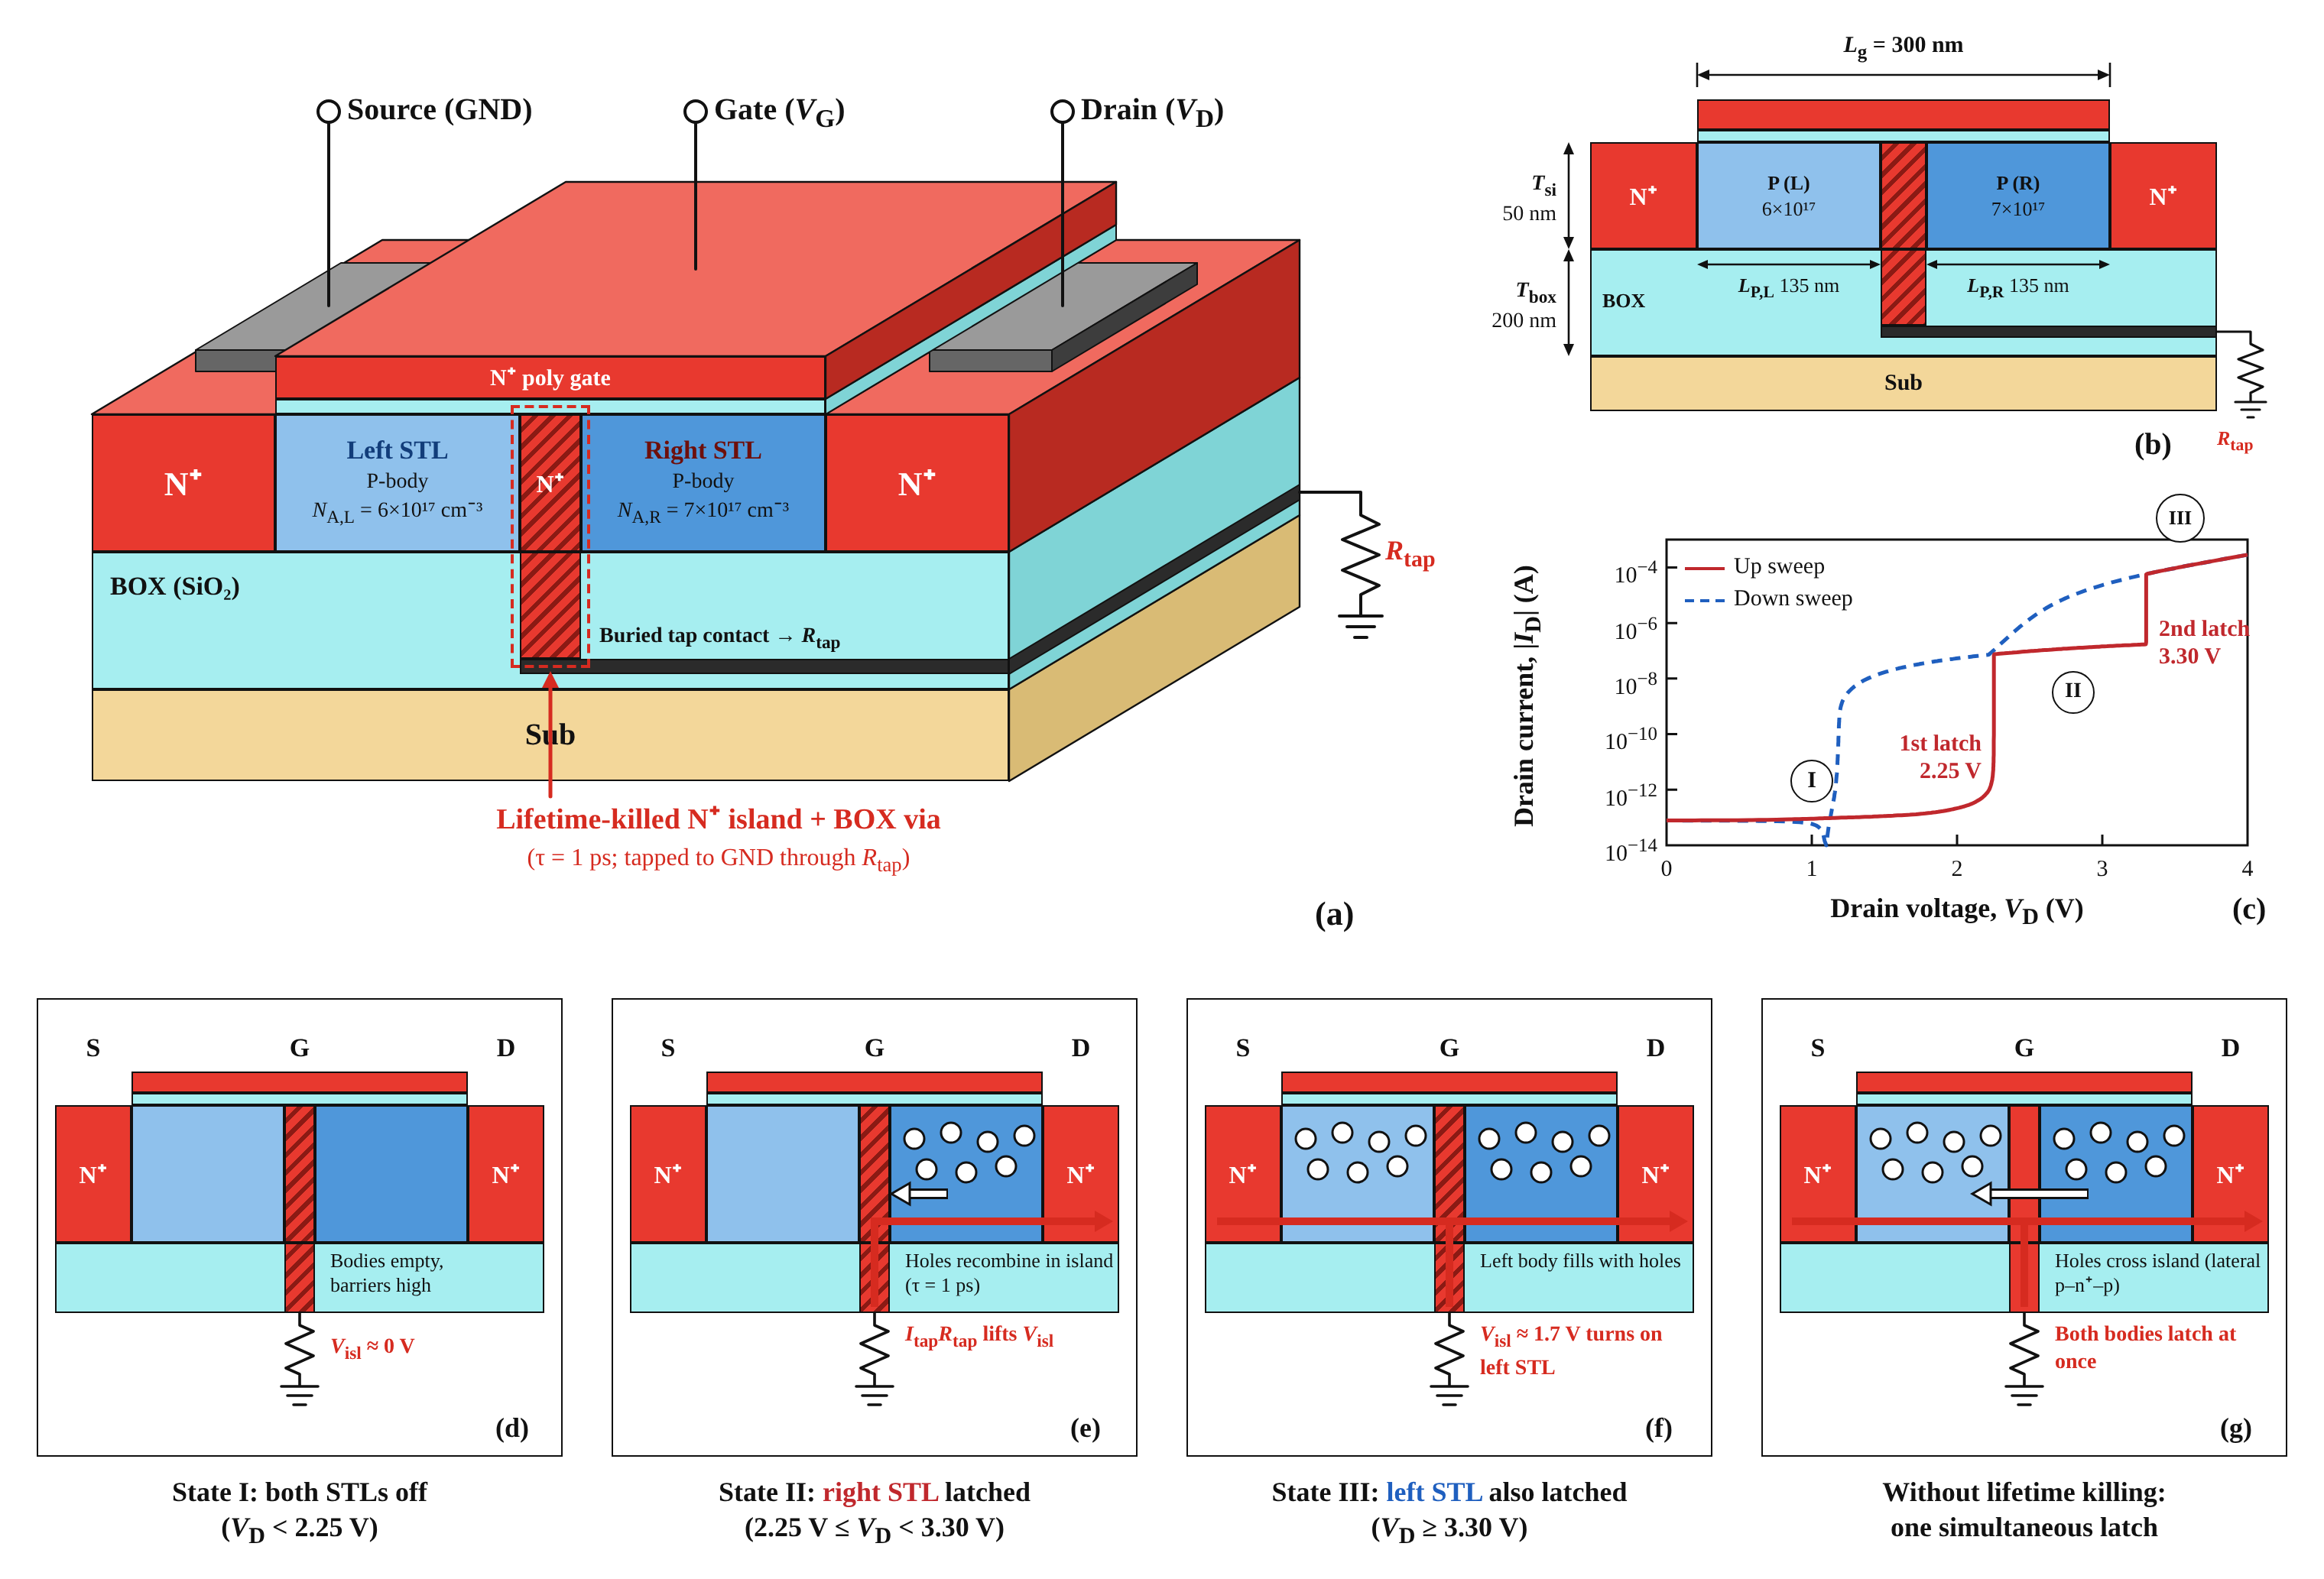
\includegraphics[width=0.92\textwidth]{fig1_concept.png}
\caption{Proposed divided-body SOI STL. (a) Left and right STLs share one gate; an n$^+$ island with a BOX via is grounded through $R_{tap}$. (b) Cross section of the reference device. (c) Two latches of the decoupled reference device (island lifetime 1~ps). (d)--(f) Body holes in states I--III. (g) Without lifetime killing, holes cross the island (lateral p-n$^+$-p) and both bodies latch at once.}
\label{fig:concept}
\end{figure*}

\section{Device and Simulation Method}
The reference device (Fig.~\ref{fig:concept}) has $L_g=300$~nm, $T_{si}=50$~nm, $t_{ox}=20$~nm, $T_{box}=200$~nm, n$^+$ S/D of $10^{20}$~cm$^{-3}$, a 30~nm n$^+$ island ($10^{20}$~cm$^{-3}$) at mid-channel, left and right p-bodies of $6\times10^{17}$ and $7\times10^{17}$~cm$^{-3}$, $V_G=-0.2$~V, $R_{tap}=10$~M$\Omega$ and a width of 0.5~$\mu$m. The island is connected through an n$^+$ via in the BOX to a bottom tap electrode. Fig.~\ref{fig:circuit} gives the equivalent circuit: each STL is a MOSFET with a parasitic n-p-n transistor on its floating body, charged by an II current source; the island node is the source of the right STL and the drain of the left STL.

Silvaco ATLAS~\cite{atlas} is used with \texttt{bgn}, \texttt{consrh}, \texttt{conmob}, \texttt{fldmob}, Fermi statistics, trap-assisted and band-to-band tunneling and the Selberherr II model~\cite{selberherr,maes}. With \texttt{consrh} the effective SRH lifetime is $\tau_{eff}=\tau_0/(1+N/N_{SRH})$, $N_{SRH}=5\times10^{16}$~cm$^{-3}$; lifetimes quoted below are the base value $\tau_0$, so $\tau_{eff}=\tau_0/2001$ in the island and $\approx\tau_0/14$ in the bodies. Adding Auger recombination changed the latch voltages by less than 2~mV. Because latching produces an S-shaped I--V on which a static voltage sweep stops at the fold, the drain is ramped in time, 0$\rightarrow$6$\rightarrow$0~V at 0.7~V/ms; the transient crosses the unstable branch and returns the jumps and hysteresis directly. Changing the ramp rate from 0.07 to 7~V/ms moves the first latch by 0.1--0.2~V and the second by less than 0.06~V. The final runs use MixedMode (device plus $R_{tap}$ and sources), which agreed with device-only runs to four digits and was 20 times faster. A latch is defined as a change of the path current by more than one decade at a fixed applied voltage (within 2~mV) that reaches a real current level; numerical artifacts are excluded by checking the time step, the KCL residual, internal potentials and the gate displacement current.

\begin{figure}[!t]
\centering
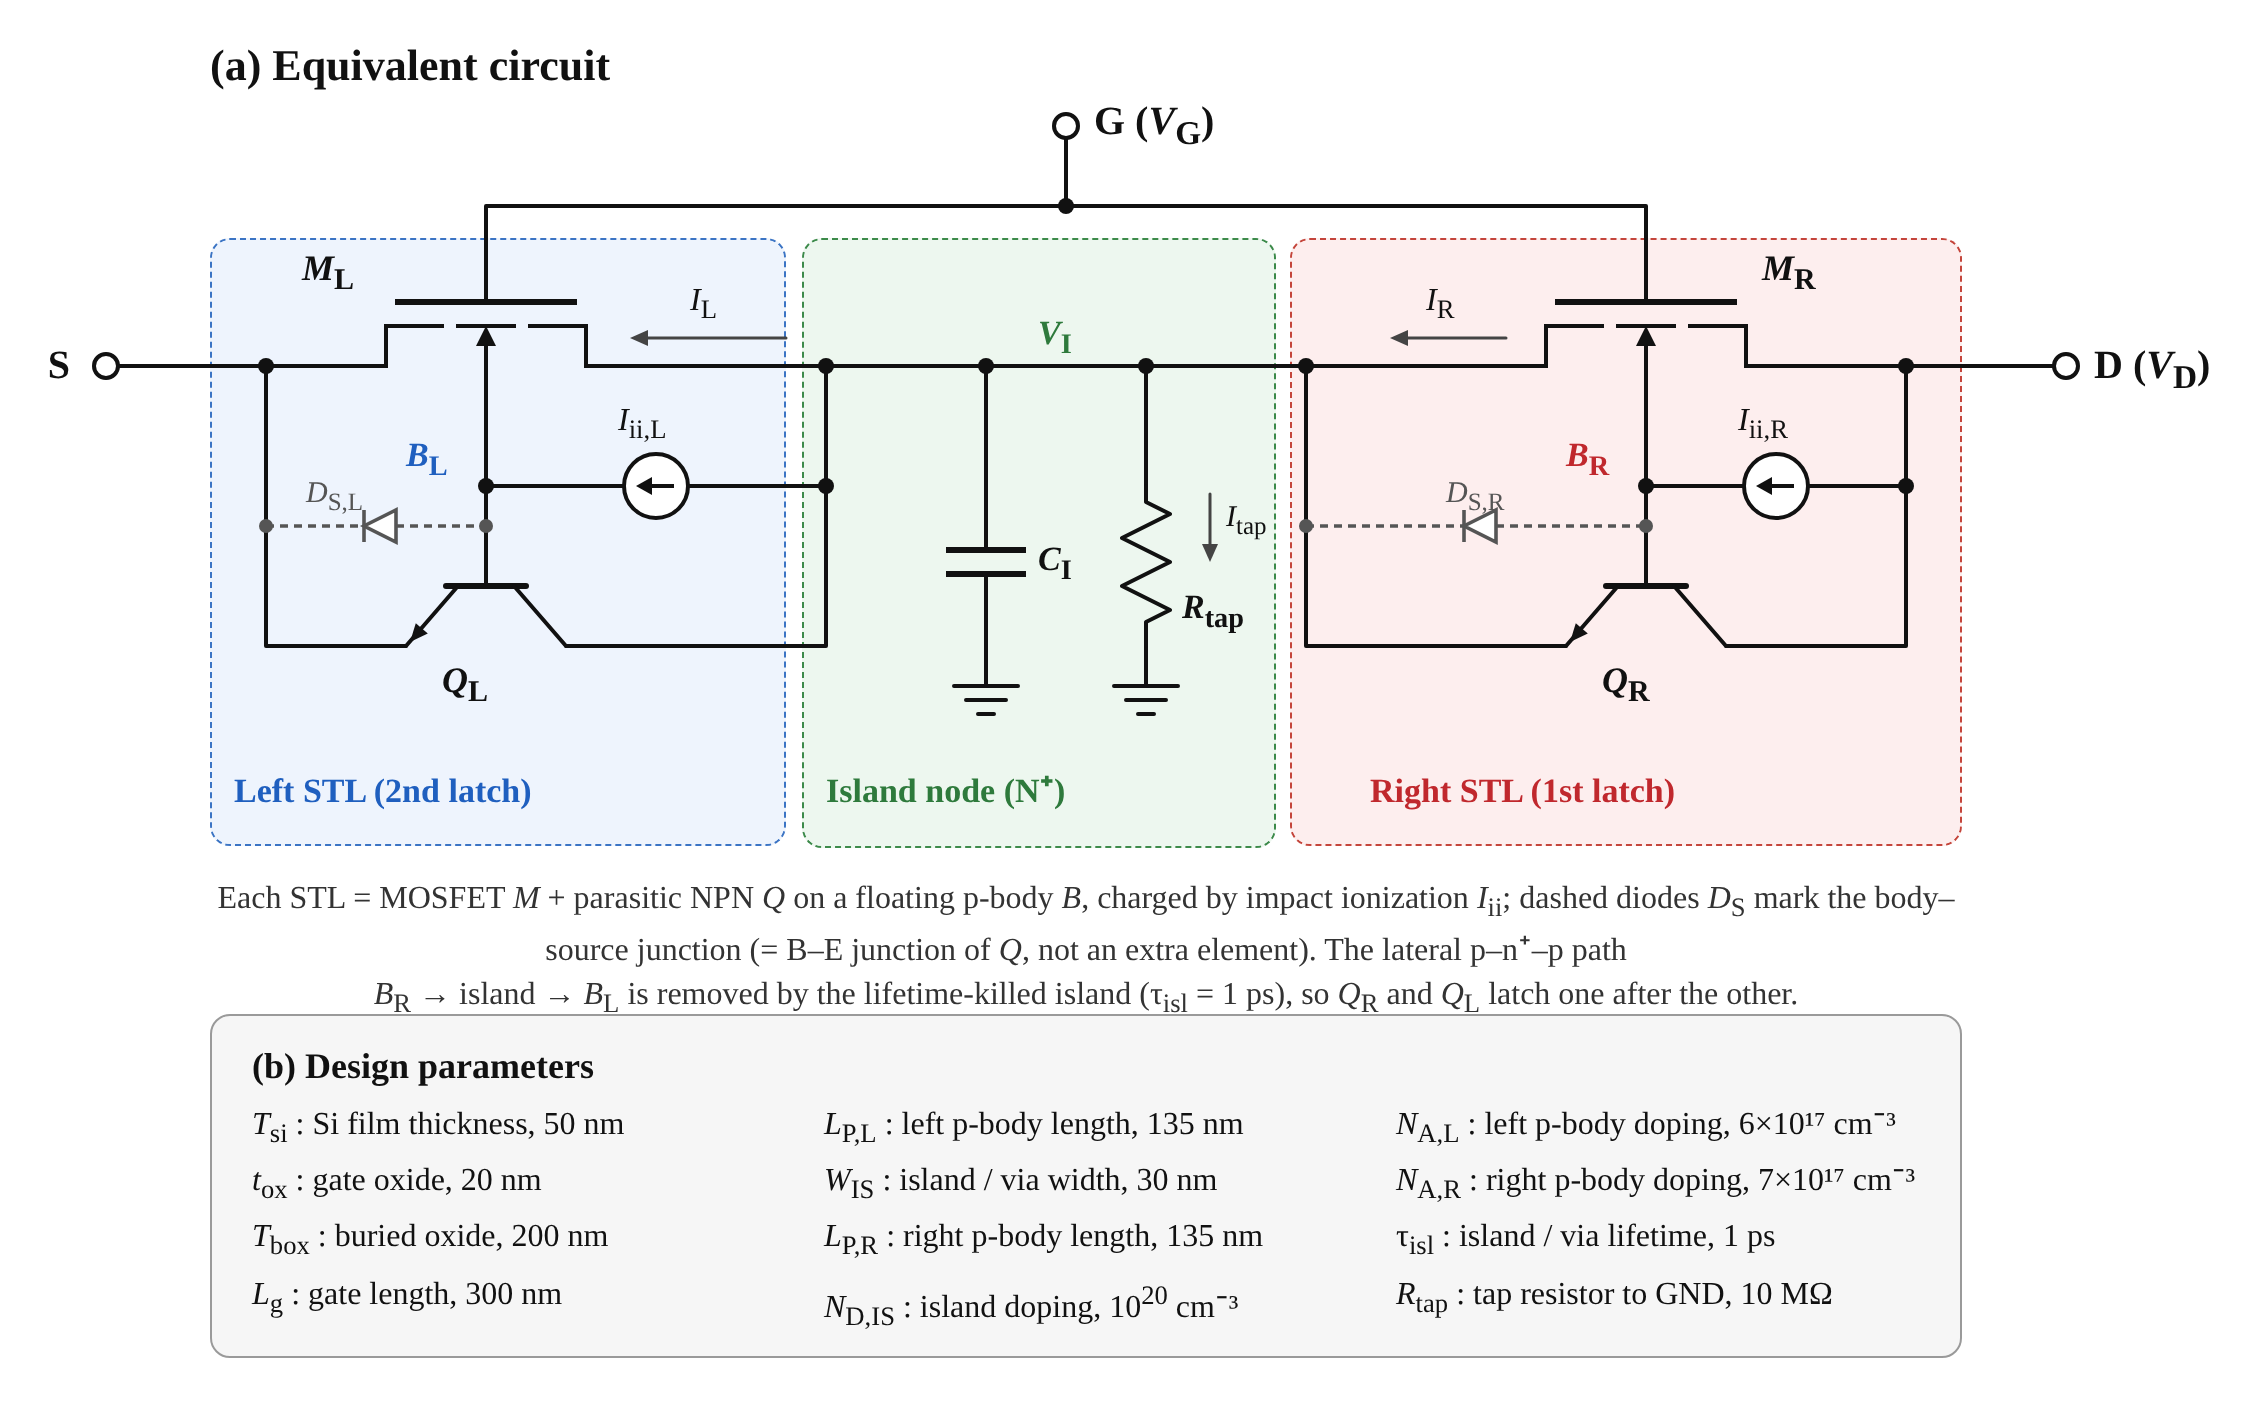
\includegraphics[width=\columnwidth]{fig2_equivalent_circuit.png}
\caption{(a) Equivalent circuit of the divided-body STL. In the decoupled device the island removes the lateral hole path; in the coupled device (Sections~V--VI) an additional body-to-body hole current source is needed. (b) Design parameters of the reference device.}
\label{fig:circuit}
\end{figure}

\section{Why the Device Latched Only Once}
Fig.~\ref{fig:evol} summarizes the structures tried before two latches were obtained. \textit{Body-doping split.} Small (4--12\%) and large (2.3--10 times) left/right doping differences in a single body always gave one latch; the hole quasi-Fermi level stayed continuous across the doping step, because a p/p$^+$ step does not block majority holes, so the two regions cannot float to different potentials. An oxide notch under the body with a thin Si bridge, a left/right $T_{si}$ split, a split gate and an n$^+$/n$^-$/p/n$^+$ stack also gave one latch. \textit{Floating island.} A 30~nm n$^+$ island separated the two body potentials before latching ($-0.02$ and 0.36~V), but both bodies and the island jumped together at 3.26~V [Fig.~\ref{fig:evol}(a)]: with a floating island the right-STL current must flow through the left STL (series constraint). \textit{Tapped island.} Grounding the island through $R_{tap}$ removed this constraint, but at $R_{tap}$ = 600, 60 and 10~k$\Omega$ the latch stayed at 2.990~V; zooming into the jump, the right body rose first and the left body followed within $\approx10$~ns [Fig.~\ref{fig:evol}(b)]. Holes injected from the right body into the 30~nm island crossed it and charged the left body: the right p-body, the island and the left p-body form a lateral p-n$^+$-p transistor. A 100~nm island still coupled the bodies, and a top ohmic contact on the island let holes pass underneath it. Only reducing the lifetime of the island and via to 1~ps left the left STL off while the right STL latched alone [Fig.~\ref{fig:evol}(c)]. Raising $R_{tap}$ to 10~M$\Omega$ then lifted the island potential enough to drive the left STL, and a standalone left STL showed that a body doping of $6\times10^{17}$~cm$^{-3}$ is needed for an abrupt latch ($3$ and $5\times10^{17}$ turned on gradually).

\begin{figure*}[!t]
\centering
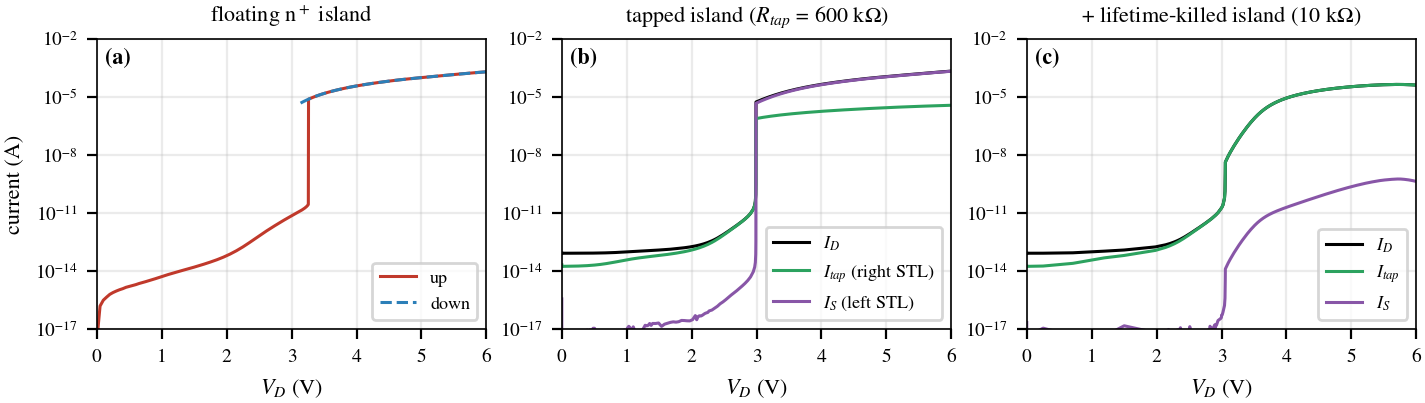
\includegraphics[width=0.86\textwidth]{fig3_evolution.png}
\caption{Latching of the intermediate structures. (a) Floating n$^+$ island: both STLs latch together at 3.26~V. (b) Island grounded through $R_{tap}=600$~k$\Omega$: the right ($I_{tap}$) and left ($I_S$) STLs jump together at 2.99~V (lateral p-n$^+$-p coupling). (c) Island lifetime 1~ps: only the right STL latches.}
\label{fig:evol}
\end{figure*}

\section{Decoupled Device: Two Latches and Their Mechanism}
With the island killed (1~ps), the reference device latches at 2.251~V (right STL; $I_{tap}$ jumps from $10^{-12}$ to $7\times10^{-8}$~A, state I$\rightarrow$II) and at 3.300~V (left STL; II$\rightarrow$III), when the island potential reaches 1.67~V, close to the latch voltage of the standalone left STL in the same model (1.78~V). On the way down the left and right STLs turn off at $\approx2.24$ and $\approx1.20$~V, so both latches have hysteresis [Fig.~\ref{fig:concept}(c)].

Twenty-eight solution snapshots were analyzed per STL: source--body electron barrier, II hole current $I_{ii}=qW\!\int G_{ii}dA$ and recombination in the body and in the n$^+$ region that acts as its source [Fig.~\ref{fig:mech}]. For the first latch the right drain-junction field is $1.16\times10^6$~V/cm ($M-1\approx0.25$); between 2.24 and 2.26~V, $I_{ii}$ jumps by four decades and the right barrier collapses from 0.60 to 0.28~eV. After latching, $I_{ii}$ equals body plus island recombination (e.g., $1.96\times10^{-8}\approx1.06\times10^{-8}+1.00\times10^{-8}$~A at 3.0~V). For the second latch the field at the left side of the island rises from $3.6\times10^5$ to $7.1\times10^5$~V/cm as the island potential rises, and between 3.28 and 3.32~V the left barrier collapses from 0.61 to 0.10~eV. The $G_{ii}$ map shows generation only at the two drain-side junctions; holes from the right body recombine in the island, so the left STL is turned on only by its own drain field. The turn-off is set by the hole margin: at $\tau_{0,Si}=10^{-7}$~s only 29\% of the generated holes recombine at the last on-point, so the latch survives to low current, whereas at $\tau_{0,Si}=10^{-8}$~s 78\% are lost and the left STL falls by six decades within 20~mV at a holding current of $5.5\times10^{-7}$~A.

Eighty-six single-parameter splits (Table~\ref{tab:knob}) show that the two latches are designed independently: the right-body doping moves the first latch (1.24--2.51~V), the left-body doping the second (2.28--4.01~V), $V_G$ moves both, and $R_{tap}$ divides the jump heights between them. With $\tau_{0,Si}=10^{-8}$~s and the island moved to 60\% of $L_g$ (left body 165~nm, right body 105~nm), the two hysteresis loops lie at 1.23--1.45~V and 2.56--4.78~V and are separated by 1.12~V. This device (island 30~nm, island lifetime 1~ps) is the decoupled reference for the rest of the paper.

\begin{figure*}[!t]
\centering
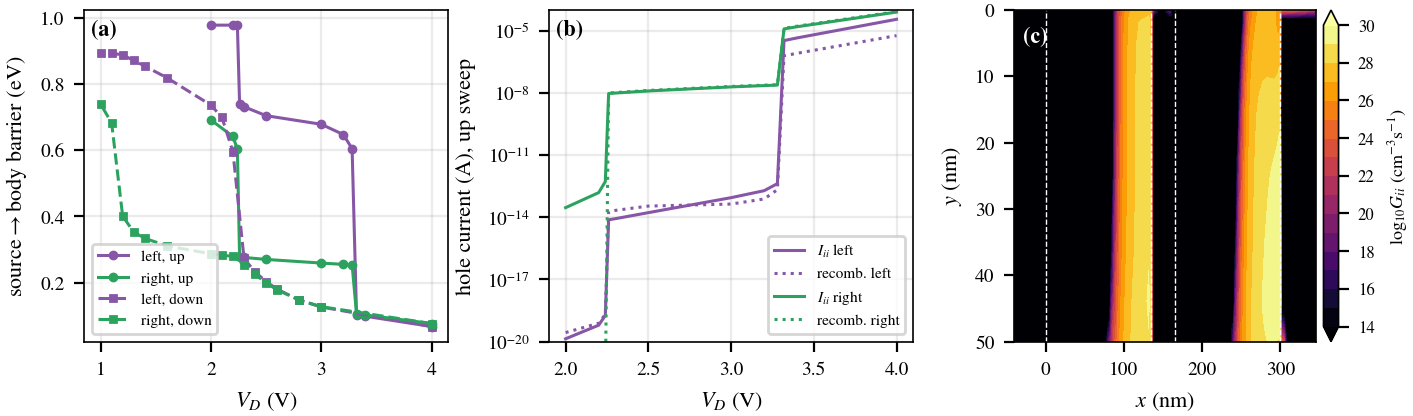
\includegraphics[width=0.84\textwidth]{fig6_mechanism.png}
\caption{Snapshot-based mechanism of the decoupled reference device ($\tau_{0,Si}=10^{-7}$~s). (a) Source-to-body electron barrier of each STL (solid: up, dashed: down). (b) II hole current (solid) and recombination (dashed) on the up sweep. (c) $G_{ii}$ map just after the second latch (3.32~V); dotted lines: source edge, island, drain edge.}
\label{fig:mech}
\end{figure*}

\begin{table}[!t]
\caption{Design Knobs of the Decoupled Device (86 DD MixedMode Splits)}
\label{tab:knob}
\centering\footnotesize
\begin{tabular}{@{}p{0.24\columnwidth}p{0.34\columnwidth}p{0.32\columnwidth}@{}}
\toprule
Knob & Effect when increased & Cost \\ \midrule
$N_{A,R}$ & 1st latch up (1.24--2.51 V) & loop spacing shrinks \\
$N_{A,L}$ & 2nd latch up (2.28--4.01 V) & no latch $\le5\times10^{17}$ \\
$V_G$ & both latches down & loop 1 narrows \\
$R_{tap}$ & larger 2nd jump & smaller 1st jump \\
$\tau_{0,Si}$ (decreased) & abrupt turn-off & both latches up \\
island toward drain & loops separate & 1st latch lost at $\ge65$\% \\ \bottomrule
\end{tabular}
\end{table}

\section{Decoupled Device Equals a Series STL Pair}
To test whether the decoupled device adds anything to a circuit, the island of the decoupled reference was replaced by a metal core through the Si film with a 10~nm n$^+$ shell (an implementable form of island recombination; first and second latch 1.499/4.616~V), and this device was then cut through the middle of the core into two independent ATLAS devices, each keeping its geometry, mesh and half of the core as its internal electrode. The two STLs were wired in series in MixedMode with the same $R_{tap}$ and gate (CUT). A realistic pair of discrete SOI MOSFETs with 500~nm n$^+$ S/D and top contacts (SD) was also simulated. CUT reproduces the one-device result within 3~mV at the second latch and 25~mV elsewhere (Table~\ref{tab:ctrl}, Fig.~\ref{fig:series}(a)); SD differs by 0.19~V only through its geometry. A divided-body device with no hole transport across the island is therefore exactly a series STL pair: the separate latches alone are not a new function, only a more compact layout.

Keeping the island lifetime at the Si value ($\tau_{0,isl}=10^{-8}$~s, ``coupled'') changes this. The second latch drops by 2.6~V to 1.969~V, and the device departs from the series circuit in three ways. First, in a series circuit each STL current is set by its own terminal voltages, so the left-STL operating point ($|I_S|$, $V_{tap}$) must lie on the I--V of a standalone left STL with the same body (Fig.~\ref{fig:series}(b), gray). The killed-island device follows that curve within 0.03~V at 1--3~mA (2.269 vs 2.272~V at 1~mA). The coupled device carries the same current at a much lower voltage (1.724~V at 1~mA; 1.519 vs 2.469~V at 3~mA). Second, above 1~mA its left-STL voltage decreases as the current increases, a negative differential resistance that a monotonic standalone on-branch cannot produce. Third, a jump appears at 3.38~V. A hole balance of each body from the snapshots (generation, recombination and $\int J_p\,dy$ at the island edges) shows that the fraction of the left-body hole supply that has crossed the island rises from 23\% at 3.0~V to 59\% at 3.5~V: the jump closes an n-p-n-p-n hole loop from the right body through the island into the left body. With the island killed this fraction is zero and the jump is absent. Because the jump is only a factor of 2.5 in current and occurs near 6~mA/$\mu$m in an isothermal simulation, it is used here only as evidence of coupling, not as a fourth state. In circuit terms (Fig.~\ref{fig:circuit}), the coupled device needs a body-to-body hole current source in addition to the $R_{tap}$ node; its magnitude is the coupling strength.

\begin{table}[!t]
\caption{Series-Circuit Control (V; Turn-Off at $|I_S|<10^{-8}$~A)}
\label{tab:ctrl}
\centering\footnotesize
\begin{tabular}{@{}lccc@{}}
\toprule
 & 1st on & 2nd on & 2nd off \\ \midrule
one device, metal core & 1.499 & 4.616 & 2.081 \\
two STLs in series (CUT) & 1.476 & \textbf{4.613} & 2.061 \\
two STLs in series (SD) & 1.471 & 4.428 & 2.019 \\
one device, coupled island & 1.444 & \textbf{1.969} & 1.747 \\ \bottomrule
\end{tabular}
\end{table}

\begin{figure*}[!t]
\centering
\includegraphics[width=0.9\textwidth]{figR_series.pdf}
\caption{Series-circuit control. (a) $|I_D|$--$V_D$ (solid: up, dashed: down) of the metal-core device, two separately simulated STLs in series (CUT, SD) and the coupled device; CUT overlaps the metal-core device. (b) Left-STL operating point ($V_{tap}$ vs $|I_S|$, down sweep) against a standalone left STL ($V_D$ vs $|I_D|$, gray). A series circuit must lie on the gray curve.}
\label{fig:series}
\end{figure*}

\section{Coupling Strength as a Design Knob}
Holes entering the n$^+$ island diffuse as minority carriers over $L_p=\sqrt{D_p\tau_{eff}}$; with $\tau_{eff}=\tau_{0,isl}/2001$ and $D_p\approx2$~cm$^2$/s, $L_p\approx32~\mathrm{nm}\times\sqrt{\tau_{0,isl}/10^{-8}~\mathrm{s}}$. The coupling should therefore scale with $L_p/W_{IS}$, and it was varied in two ways from the reference: (i) the island lifetime $\tau_{0,isl}=10^{-12}$--$10^{-8}$~s at $W_{IS}=30$~nm (only the two lifetime lines of the deck differ), and (ii) the island width $W_{IS}=15$--200~nm at $\tau_{0,isl}=\tau_{0,Si}=10^{-8}$~s. The width sweep keeps both body lengths and widens only the island, so $L_g=270~\mathrm{nm}+W_{IS}$ grows with it; a killed island at $W_{IS}=120$~nm separates this gate-length effect.

The results are listed in Table~\ref{tab:couple} and Fig.~\ref{fig:knob}. The first latch (right STL) stays at 1.444--1.449~V in every case; only the second latch moves. In the lifetime sweep it stays at 4.74--4.78~V (series circuit) up to $\tau_{0,isl}=10^{-10}$~s and falls to 2.99~V at $10^{-9}$~s and 1.97~V at $10^{-8}$~s. In the width sweep it falls from 4.31~V (200~nm) through 3.34, 2.58, 2.19 and 2.06 to 1.97~V (30~nm). The two sweeps fall on one curve versus $L_p/W_{IS}$ [Fig.~\ref{fig:knob}(b)]; at equal $L_p/W_{IS}$ they differ by at most $\approx0.3$~V, which we attribute to the one-dimensional diffusion picture behind $L_p/W_{IS}$. Killing the 120~nm island gives 4.761/2.577~V, the same as the killed 30~nm island (4.779/2.565~V), although $L_g$ grows from 0.30 to 0.39~$\mu$m; the width dependence of the coupled devices is therefore entirely due to coupling. The island width, a mask dimension, is the practical knob, whereas the lifetime knob needs a local, extreme lifetime control.

\begin{table}[!t]
\caption{Second Latch Versus Coupling Strength. On/Off: One-Decade Jump at Fixed Applied Voltage (V); Jump: Decades of $|I_D|$ at Turn-On}
\label{tab:couple}
\centering\scriptsize\setlength{\tabcolsep}{3pt}
\begin{tabular}{@{}lccccc@{}}
\toprule
 & $L_p/W_{IS}$ & 2nd on & 2nd off & hyst. & jump \\ \midrule
$W_{IS}$ = 15~nm & 2.13 & cont.$^a$ & same curve & 0 & none \\
30~nm ($\tau_{0,isl}=10^{-8}$~s) & 1.07 & 1.969 & 1.956 & 0.01 & 0.8 \\
45~nm & 0.71 & 2.064 & 1.997 & 0.07 & 1.3 \\
60~nm & 0.53 & 2.193 & 2.019 & 0.17 & 1.8 \\
90~nm & 0.36 & 2.579 & 2.037 & 0.54 & 2.5 \\
120~nm & 0.27 & 3.339 & 2.040 & 1.30 & 3.2 \\
200~nm & 0.16 & 4.314 & 2.041 & 2.27 & 4.1 \\ \midrule
$\tau_{0,isl}=3\times10^{-9}$~s (30~nm) & 0.58 & 2.277 & 2.179 & 0.10 & 1.4 \\
$10^{-9}$~s & 0.34 & 2.985 & --$^b$ & -- & -- \\
$10^{-10}$~s & 0.11 & 4.742 & 2.526 & 2.22 & 3.7 \\
$10^{-11}$~s & 0.03 & 4.776 & 2.562 & 2.21 & 3.7 \\ \midrule
killed ($10^{-12}$~s), 30~nm & 0.01 & 4.779 & 2.565 & 2.21 & 3.7 \\
killed, 120~nm & 0.003 & 4.761 & 2.577 & 2.18 & 3.6 \\ \bottomrule
\end{tabular}\\[2pt]
{\raggedright\scriptsize $^a$ Continuous turn-on between 1.86 and 2.0~V. $^b$ Run stopped at 5.45~V (time limit).\par}
\end{table}

\begin{figure*}[!t]
\centering
\includegraphics[width=\textwidth]{figS_knob.pdf}
\caption{Continuous tuning of the coupling. (a) Left-STL current of the width sweep (solid: up, dashed: down; black: 120~nm, island killed). (b) Second-latch turn-on (filled) and turn-off (open) versus $L_p/W_{IS}$: red, width sweep; blue, island-lifetime sweep; $\times$, killed islands (30, 120~nm); the bar marks the continuous turn-on at 15~nm. (c) Second-stage hysteresis (0 at 15~nm). (d) Deviation of the left-STL operating point from the series circuit (standalone left STL) at $|I_S|$ = 3~mA (solid) and 1~mA (dotted), down sweep.}
\label{fig:knob}
\end{figure*}

\textit{Hysteresis.} The second turn-off stays at 2.00--2.04~V for all coupled widths from 45 to 200~nm, so the width moves only the turn-on and the second-stage hysteresis is tuned continuously from 2.27~V to zero [Fig.~\ref{fig:knob}(c)]. The low turn-off is itself a coupling effect: at the same 120~nm geometry the left STL turns off at 2.04~V with a coupled island and at 2.58~V with a killed one. The 3.0~V hole maps (Fig.~\ref{fig:holes}) show why. Both devices are inside their hysteresis at 3.0~V, with an empty left body on the way up and a filled one on the way down; the difference is the island. The coupled island holds $10^{16}$--$10^{17}$~cm$^{-3}$ holes on the way down and keeps feeding the left body, whereas the killed island stays below $10^{4}$~cm$^{-3}$. A wide island blocks the coupling before latch-on, but after latch-on the hole flux across it is large and the coupling returns, holding the left STL down to a lower voltage. The right-STL turn-off moves in the same direction (1.035~V coupled vs 1.228~V killed).

\textit{Limit of strong coupling.} Coupling has a cost: the height of the second jump falls from 4.1 decades (200~nm) through 3.2, 2.5, 1.8 and 1.3 to 0.8 decades (30~nm), and at 15~nm the left STL turns on without a jump between 1.86 and 2.0~V and returns along the same curve ($|I_S|=5.2\times10^{-6}$~A up and down at 2.0~V). The two bodies then behave as one hole reservoir [Fig.~\ref{fig:holes}, bottom]. The useful range for an abrupt second latch therefore starts between 15 and 30~nm; we take 30--120~nm as the tuning range and treat 200~nm, where the island is wider than either body, as the limit toward zero coupling. The hole-loop jump remains at 3.10--3.15~V at 15~nm.

\textit{Deviation from the series circuit.} Applying the operating-point test of Fig.~\ref{fig:series}(b) to every run [Fig.~\ref{fig:knob}(d)], the left-STL voltage at 3~mA lies $-1.29$, $-0.95$, $-0.70$, $-0.53$, $-0.31$, $-0.22$ and $-0.11$~V from the standalone characteristic for $W_{IS}$ = 15, 30, 45, 60, 90, 120 and 200~nm, and returns to $-0.03$ and $+0.07$~V when the 30 and 120~nm islands are killed. The lifetime sweep lies on the same curve ($-0.47$~V at $L_p/W_{IS}=0.58$ vs $-0.53$~V for 60~nm at 0.53). Between 1 and 10~$\mu$A all runs are within $\pm0.13$~V, i.e., the coupling shows once the left STL is strongly on and the hole flux across the island is large. The departure from a series STL pair thus holds over the whole tuning range, and its size is set by the coupling strength.

\begin{figure}[!t]
\centering
\includegraphics[width=\columnwidth]{figT_holes.pdf}
\caption{Hole density in the Si film from solution snapshots (dotted: source edge, island edges, drain edge). Top: $W_{IS}=120$~nm, coupled; middle: 120~nm, killed; 3.0~V on the up (left) and down (right) sweep. Bottom: 15~nm, coupled, 2.5~V.}
\label{fig:holes}
\end{figure}

\section{Discussion}
\textit{Implementation.} The two ends of the coupling range have different physical forms. Zero coupling needs an island effective lifetime of $\le5\times10^{-14}$~s, which damage alone is unlikely to provide; a metal or silicide core through the full Si thickness gives the same result (Section~V; with $\tau_{0,Si}=10^{-8}$~s and the island at 60\%), but it was modeled as an ideal ohmic boundary with infinite surface recombination. Intermediate coupling is obtained simply by the island width at the Si lifetime, so no local lifetime control of the island is needed. The body lifetime of $\tau_{0,Si}=10^{-8}$~s used for abrupt turn-off is within conventional lifetime control (Au/Pt diffusion, electron or proton irradiation)~\cite{kim_lifetime}, and $R_{tap}$ = 1--10~M$\Omega$ can be a high-resistance poly-Si resistor. The decoupled layout is shorter than a stacked series pair because the island node is taken out through the BOX instead of a top contact, at the cost of a BOX via and back-side wiring.

\textit{Use of the coupling knob.} With the first latch fixed, the coupling sets where the second latch fires and how wide its hysteresis is. A wide second-stage window (weak coupling) suits a three-state memory or a ternary threshold element; a narrow window (strong coupling) gives a second, nearly reversible switching step. The decoupled device behaves as a series pair, so circuit models of series STLs, including current-driven relaxation oscillation, apply directly; for the coupled device the island node needs the additional body-to-body hole current, which we have not yet modeled.

\textit{Limitations.} All results are 2D, isothermal drift-diffusion. Local-field II overestimates generation in short channels: in the standalone left STL the energy-balance (hydrodynamic) latch was 0.7--0.8~V higher than the DD one. Full-device energy-balance runs stopped at 3.6--5.3~V because the electron temperature at the right drain junction exceeded $10^4$~K and the time step collapsed, despite coupled Newton, a 1~nm mesh, relaxed tolerances, MixedMode and graded drains; the second latch is therefore a DD result. An attempt to calibrate the II coefficients to a measured double-latch bulk device~\cite{noh_triristor} matched its Id--Vg but not its first latch, and a 20\% change of the Selberherr $B$ coefficient moved a coefficient-sensitive latch by $\approx$20\%. Absolute voltages are thus uncertain by roughly $\pm$20\%, whereas the comparisons in this paper (coupled vs killed vs series circuit at the same model) do not depend on the coefficients. Self-heating at the mA/$\mu$m currents of state III is not included.

\section{Conclusion}
A divided-body SOI STL with a resistively grounded n$^+$ island latches twice once hole transport across the island is removed, and each latch is the point where II hole generation in one body overcomes recombination. Such a decoupled device is, however, a series STL pair: two separately simulated STLs in series reproduce it within 25~mV. What a single device adds is the hole coupling between the bodies. The coupled device departs from the series characteristic by up to 1.29~V at 3~mA, shows negative differential resistance and a hole-loop jump, and its coupling is tuned continuously by the island lifetime or, more practically, the island width; both collapse onto $L_p/W_{IS}$. With the first latch fixed at 1.44--1.45~V, the second latch spans 1.97--4.78~V and the second-stage hysteresis 0--2.27~V, without a gate-length effect. The strongest coupling (15~nm) removes the second latch and sets the lower bound of the useful width. Remaining work is a compact model of the body-to-body hole current, energy-balance confirmation of the second latch and calibration against measured SOI devices.

\section*{Acknowledgment}
This work started as a course project of EE762 at KAIST.

\begin{thebibliography}{99}
\bibitem{chen_stl} C.-D. Chen, M. Matloubian, R. Sundaresan, B.-Y. Mao, C. C. Wei, and G. P. Pollack, ``Single-transistor latch in SOI MOSFETs,'' \emph{IEEE Electron Device Lett.}, vol.~9, no.~12, pp.~636--638, Dec. 1988.
\bibitem{han_biristor} J.-W. Han and Y.-K. Choi, ``Biristor---Bistable resistor based on a silicon nanowire,'' \emph{IEEE Electron Device Lett.}, vol.~31, no.~8, pp.~797--799, Aug. 2010.
\bibitem{kim_1tdram} D.-O. Kim, D.-I. Moon, and Y.-K. Choi, ``Optimization of bias schemes for long-term endurable 1T-DRAM through the use of the biristor mode operation,'' \emph{IEEE Electron Device Lett.}, vol.~35, no.~2, pp.~220--222, Feb. 2014.
\bibitem{moon_fin} D.-I. Moon, S.-J. Choi, J.-W. Han, S. Kim, and Y.-K. Choi, ``Fin-width dependence of BJT-based 1T-DRAM implemented on FinFET,'' \emph{IEEE Electron Device Lett.}, vol.~31, no.~9, pp.~909--911, Sep. 2010.
\bibitem{han_lif} J.-W. Han and M. Meyyappan, ``Leaky integrate-and-fire biristor neuron,'' \emph{IEEE Electron Device Lett.}, vol.~39, no.~9, pp.~1457--1460, Sep. 2018.
\bibitem{han_mimic} J.-K. Han \emph{et al.}, ``Mimicry of excitatory and inhibitory artificial neuron with leaky integrate-and-fire function by a single MOSFET,'' \emph{IEEE Electron Device Lett.}, vol.~41, no.~2, pp.~208--211, Feb. 2020.
\bibitem{han_sciadv} J.-K. Han \emph{et al.}, ``Cointegration of single-transistor neurons and synapses by nanoscale CMOS fabrication for highly scalable neuromorphic hardware,'' \emph{Sci. Adv.}, vol.~7, no.~32, Art. no. eabg8836, Aug. 2021.
\bibitem{kim_osc} H.-Y. Kim, S.-I. Kim, J.-K. Han, J.-W. Jung, and Y.-K. Choi, ``A single MOSFET-based oscillator on a bulk-silicon wafer,'' \emph{IEEE Electron Device Lett.}, vol.~45, no.~1, pp.~8--11, Jan. 2024.
\bibitem{lee_1v} S.-W. Lee \emph{et al.}, ``Single transistor latch near 1~V with asymmetric biasing in a MOSFET,'' \emph{IEEE Trans. Electron Devices}, vol.~71, no.~11, pp.~6539--6543, Nov. 2024.
\bibitem{han_ptmos} J.-A. Han, J.-W. Lee, J.-K. Han, D.-W. Kim, D.-H. Lee, and Y.-K. Choi, ``P-type ternary logic MOSFET with tunable middle state using bidirectional threshold switching,'' \emph{IEEE Electron Device Lett.}, vol.~46, no.~1, pp.~16--19, Jan. 2025.
\bibitem{han_bts} J.-K. Han, J.-M. Yu, S.-Y. Nam, and Y.-K. Choi, ``CMOS ternary logic with a biristor threshold switch for low static power consumption,'' \emph{IEEE Electron Device Lett.}, vol.~43, no.~7, pp.~1005--1008, Jul. 2022.
\bibitem{jeong_tcmos} J. W. Jeong \emph{et al.}, ``Tunnelling-based ternary metal--oxide--semiconductor technology,'' \emph{Nature Electron.}, vol.~2, no.~7, pp.~307--312, Jul. 2019.
\bibitem{heo_nbo2} S. Heo \emph{et al.}, ``High-speed ternary CMOS inverter by monolithic integration of NbO$_2$ threshold switch with MOSFET,'' in \emph{IEDM Tech. Dig.}, Dec. 2021, pp.~32.2.1--32.2.4.
\bibitem{son_fbfet} J. Son, K. Cho, and S. Kim, ``New ternary inverter with memory function using silicon feedback field-effect transistors,'' \emph{Sci. Rep.}, vol.~12, Art. no. 12907, Jul. 2022.
\bibitem{kim_spti} H.-Y. Kim, H.-B. Noh, H.-Y. Maeng, and Y.-K. Choi, ``A selective positive ternary inverter using the mirror symmetry of a MOSFET with a gate--body diode,'' \emph{IEEE Trans. Electron Devices}, vol.~73, no.~8, pp.~5232--5238, Aug. 2026.
\bibitem{noh_triristor} H.-B. Noh \emph{et al.}, ``A triristor with tri-stable states using double latches,'' \emph{IEEE Electron Device Lett.}, vol.~46, no.~8, pp.~1269--1272, Aug. 2025.
\bibitem{kim_lifetime} S. Kim, S.-J. Choi, D.-I. Moon, and Y.-K. Choi, ``Carrier lifetime engineering for floating-body cell memory,'' \emph{IEEE Trans. Electron Devices}, vol.~59, no.~2, pp.~367--373, Feb. 2012.
\bibitem{maes} W. Maes, K. De Meyer, and R. Van Overstraeten, ``Impact ionization in silicon: A review and update,'' \emph{Solid-State Electron.}, vol.~33, no.~6, pp.~705--718, Jun. 1990.
\bibitem{selberherr} S. Selberherr, \emph{Analysis and Simulation of Semiconductor Devices}. Vienna, Austria: Springer-Verlag, 1984.
\bibitem{atlas} Silvaco Inc., \emph{Atlas User's Manual}, version 5.32.1.R, Santa Clara, CA, USA.
\end{thebibliography}

\end{document}
